% !TeX root = ../report.tex

\section{Trident Ray Theory} \label{sec:trident_theory}

Currently, there are many existing ray tracing algorithms for High-Intensity Focused Ultrasound simulation. Most of them aim at computing the powerloss density (heat production) or intensity from beams of rays casted from transducer. Two existing methods will be introduced briefly because they are the inspiration of the method used in this study.

The first method is to sum over all rays (set $\Phi$) that pass through a grid cube. Their energy loss in the cube is:

\begin{equation} \label{eq:first_rc}
    H = \sum_{a \in \Phi} (P(r_{a,in}) - P(r_{a,out})) = \sum_{a \in \Phi} P(r_{a,in})(1-e^{-2\alpha ||r_{a,in} - r_{a,out}||})
\end{equation}

Where $H$ is the total powerloss by all rays in the sampling grid. To obtain the powerloss density $Q$ (in $watt/m^3$), $H$ needs to be divided by volume. For each ray in $\Phi$, the algorithm needs to calculate the position where it enters and leaves a gridbox. This method cannot handle the situation where intersections are present.

In the second method, the rays are grouped into paths. Note that here same path only means that the rays start from the same transducer element, pass through the media in the same order and have the same properties such as wave type. Ray with the same path are treated as a bundle ($b$). Take the situation in Figure \ref{fig:one_gridbox} for example, the the value of the intensity loss for the all the rays that follow the same path $b$ can be calculated from:

\begin{equation} \label{eq:calc_I_Loss}
    I_{loss,b}(\vec{r_c})=\sum_{a \in b} \frac{||\vec{r}_{a,in}-\vec{r}_{a,out}||}{\Delta V} P(\vec{r}_{a,in})
\end{equation}

From intensity loss $I_{loss}$, pressure generated by all the rays in the same path $b$ can be calculated from:

\begin{equation} \label{eq:pressure_calculation}
    p_b(\vec{r}_c)=\sqrt{2\cdot Z\cdot I_{loss,b}(\vec{r}_c)e^{i\bar{\phi}_b}}
\end{equation}

Accumulate the contributionof all the possible bundles ($U$):

\begin{equation} \label{eq:sum_all_bundle}
    p_{tot}(\vec{r}_c)=\sum_{b \in U}p_b(\vec{r}_c)
\end{equation}

Accroding to Modena et al \cite{Modena_2018}, the fluid heat production is given by:

\begin{equation} \label{eq:fluid_hp}
    Q(\vec{r})=\frac{\alpha}{Z}|p_{tot}|^2
\end{equation}

\begin{figure}
    \centering
    \begin{subfigure}[b]{0.45\textwidth}
        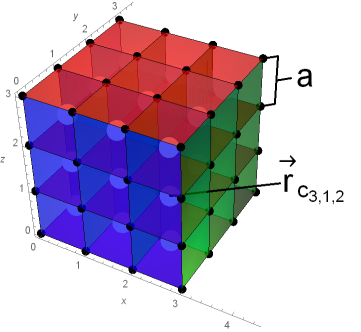
\includegraphics[width=\textwidth]{gridbox}
        \caption{}
        \label{fig:gridbox}
    \end{subfigure}
    %
    \begin{subfigure}[b]{0.5\textwidth}
        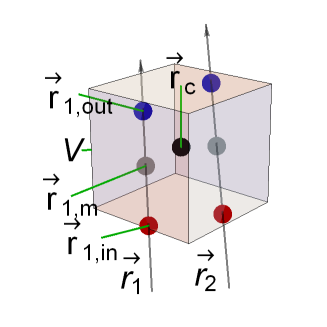
\includegraphics[width=\textwidth]{one_gridbox}
        \caption{}
        \label{fig:one_gridbox}
    \end{subfigure}
    \caption{(a) An example of Axis-Aligned Bounding Box (AABB) where $r_{c_{3,1,2}}$ is the center of the box $[3,1,2]$ (b) single box with intersection, $r_1$ enters the box at $r_{1,in}$ and exit at $r_{1,out}$, similar for $r_2$}
\end{figure}

By combining the equations \ref{eq:calc_I_Loss}, \ref{eq:pressure_calculation}, \ref{eq:sum_all_bundle}, \ref{eq:fluid_hp}, we can arrive at the equation for heat production calculated from ultrasonic rays.

\begin{equation} \label{eq:heat_production_final1}
    Q(\vec{r}_c)=\frac{2\alpha}{V}\left|\sum_{b \in U}\sqrt{(\sum_{a \in U_b}P(\vec{r}_{a,in})\left\|\vec{r}_{a,in}-\vec{r}_{a,out}\right\|)} e^{i\bar{\phi}_b}\right|^2
\end{equation}

The flow of acoustic power from each transducer element is described by a number of rays\cite{sonavelle}. With more rays being sent out in the simulation, the intersection of each box tends to converge to a stable ratio. As can be seem from equation \ref{eq:heat_production_final1},in order to obtain the powerloss density, first, the impact of all the rays are accumulated within every path (bundle). For every path, their contribution is calculated in the outer summation. In a HIFU simulation, there can be many bundles due to reflection and refraction of the rays. This will cause the computation to be very expensive when a large number of rays are utilized to approximate the real intensity. 

A new idea is proposed by Prof. Huub ten Eikelder that instead of casting a large number of rays from the transducer to approximate the intensity, one can use the "trident" rays, each of which is the combination of three rays to keep track of the divergence of the beam. One of the three rays carrys the power information, the other two only serve as auxiliary rays. These three rays have almost identical paths and the geometrical spreading can be used as the divergence of the ray pattern Figure \ref{fig:Trident_ray}. At any sampling point, a plane perpendicular to the power carrying ray is created to intersect the three rays. The area of the triangle formed by the three intersection points is $S_1$ and can be used as how much the beam has spreaded. The power on a point on the ray is given by attenuation equation $P_1=P_0\cdot e^{-2\cdot \alpha \cdot r}$. Hence, the intensity and powerloss density can be derived from:
\begin{equation}
    I=\frac{P_1}{S_1}
\end{equation}
The standard way to calculte powerloss is:
\begin{equation}
    Q=2\alpha I
\end{equation}

As the length on the ray increases, the area increases quadratically as well as the divergence of the beam. In theory, it requires only one ray per bundle to determine the intensity from this bundle. This method can achieve similar pricision with less rays, compared with the first method because it only requires that there's at least one intersection with the box per bundle.

However, in real simulation, it seldom happens that there's only one ray from a bundle that intersects a box. The contribution of the bundle to the pressure in this box will then be the average pressure from these rays. More detailed discuss is available in section \ref{sec:measurement}.

\begin{figure}[h]
    \centering
    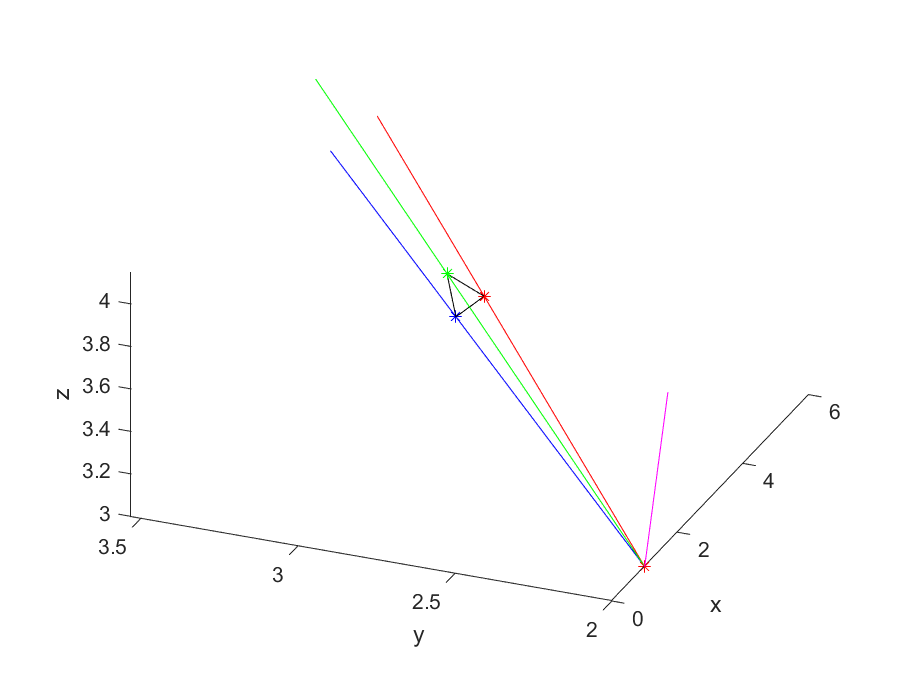
\includegraphics[width=0.6\textwidth]{trident.eps}
    \caption{An example of trident rays, the angle between rays are larger for demonstration purpose.}
    \label{fig:Trident_ray}
\end{figure}

%%%%%%%%%%%%%%%%%%%%%%%%%%%%%%%%%%%
\section{Components of HIFU Model} \label{sec:components}

A MR-HIFU system is a highly sophisticated system with many components. For simplicity reasons, the MR-HIFU system is modelled as being composed of only transducer, media, rays and sampling box. The model uses the actual geometry of phase array used in the Philips Sonavelle system \cite{sonavelle}, which consists of 256 elements placed on a spherical shell (12 cm radius of curvature and 13 cm aperture) operating at 1.4 MHz. The focus point created by this system is cigar shaped with dimensions of approximately 2mm width and 7mm length. The power of the transducer can be set as a parameter in the model, in this study, 256 watt (1 watt per transducer) is used as the total power of the transducer. 

\begin{table}[h!]
    \centering
    \begin{tabular}{c c c c c c c c} 
        \hline
        Medium & \textit{TH} & $c$ & $\rho$ & $\alpha$ & $c_p$ & $k$ \\ [0.5ex] 
        \hline\hline
        Oil & - & 1430 & 1070 & 1.04 & 4200 & 0.5 \\
        \hline
        Gel pad & 15 & 1580 & 1030 & 0.8 & 3600 & 0.65 \\
        \hline
        Skin & 2 & 1610 & 1200 & 50 & 3600 & 0.56 \\
        \hline
        Muscle & 10 & 1547 & 1050 & 9.8 & 3600 & 0.56 \\
        \hline
        Bone & - & 3736/1995 & 2025 & 1.9/2.8 & 3720 & 0.487 \\
        \hline
        Liver & - & 1578 & 1050 & 5.65 & 3600 & 0.56 \\
        \hline
    \end{tabular}
    \caption{Properties of the materials used in this study. \textit{TH}: thickness,  $c$: speed of sound, $\rho$: density,  $\alpha$: attenuation, $c_p$: specific heat capacity, $k$: thermal conductivity. \cite{Modena_2018} \cite{markoil}}
    \label{tb:media_property}
\end{table}

The transducer is submerged in Markoil which has a very low attenuation factor for ultrasonic power (Figure \ref{fig:submerged_transducer}). The acoustic property of markoil is given by Ramaekers et al \cite{markoil}. The markoil is separated from the air by a thin membrane. The model simplifies the media to consist of only bone and muscle. Skin and other soft tissues have very close properties to that of the muscle and thus not discriminated. For ultrasonic wave, the muscle and the skin behave as liquid and the bone behaves as solid. Propagation of shear (tranversal) wave is only possible in solid. Markoil is the initial medium of the trident rays. 

\begin{figure}[h]
    \centering
    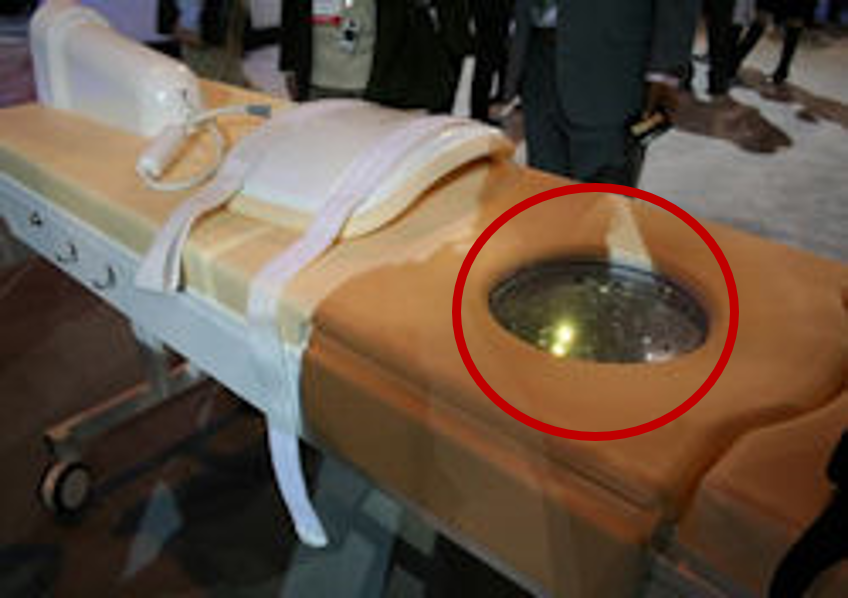
\includegraphics[width=0.5\textwidth]{transducer_markoil}
    \caption{Transducer element submerged in markoil (annotated) \cite{sonavelle} \cite{vanwijk2013}.}
    \label{fig:submerged_transducer}
\end{figure}

To measure the power production in the media caused by the ultrasound, a sampling box is employed (Figure \ref{fig:sampling_box}). Sampling is a very time consuming process, thus the sampling box is only around the focus region, which would also be the lesion area in therapeutic application. The box is divided into smaller lattices (cubes). The smaller the lattices are, the finer the resolution (Figure \ref{fig:gridbox}). The edges of the lattices should be larger than the ultrasound wave length. Two measurement methods are implemented. The first one uses the projection of the center of the lattices on the ray as the length to calculate intensity and add the intensity of all the rays together. The secound method differs the first method only in that the summation is weighted based on the length of the intersection of the ray with the lattices.

\begin{figure}[h]
    \centering
    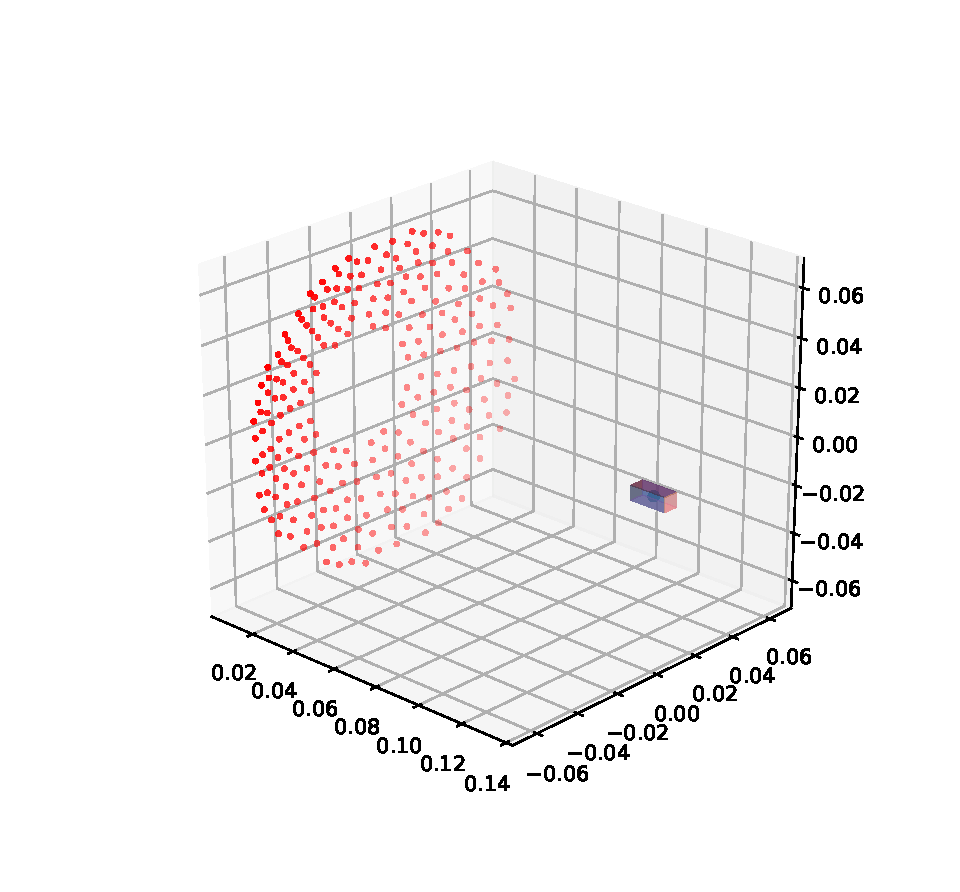
\includegraphics[width=0.6\textwidth]{sampling_box}
    \caption{Sampling box with transducer.}
    \label{fig:sampling_box}
\end{figure}

As explained in Section \ref{sec:trident_theory}, the ray in this model consists of three closely aligned rays. One ray carrys the power and is referred to as "power ray". The other two rays only helps to determine the divergence of the beam and is referred to as "auxiliary ray". The angle between any two rays of the three is referred to as "trident ray".

%%%%%%%%%%%%%%%%%%%%%%%%%%%%%%%%%%%%%
\section{Implementation of the Model} \label{sec:implement}
The mathematical model is written in Python programming language, using scipy suite\cite{scipy}. The visualization of the model is made possible with matplotlib \cite{matplotlib}. The model is produced as a python package \texttt{pyHIFU} and is available online. The four components mentioned in section \ref{sec:components} will be introduced in detail. A Python class is implemented for each component. This make the program more intuitive and easy to maintain. Other than these four component, the geometry, acoustics are also implemented in object-oriented manner. Class \texttt{HIFU} encapsulates several methods for manipulating the four components above. As is shown in Figure \ref{fig:uml_overview}, \texttt{transducer} casts \texttt{ray} at \texttt{media} and grouped them into bundle according to their properties and history. Then, the grouped rays are sampled on \texttt{box} to get the resulted pressure. The same routine is run for all the transducers. The final result is the summation of the result from all transducer.

\begin{figure}[h]
    \centering
    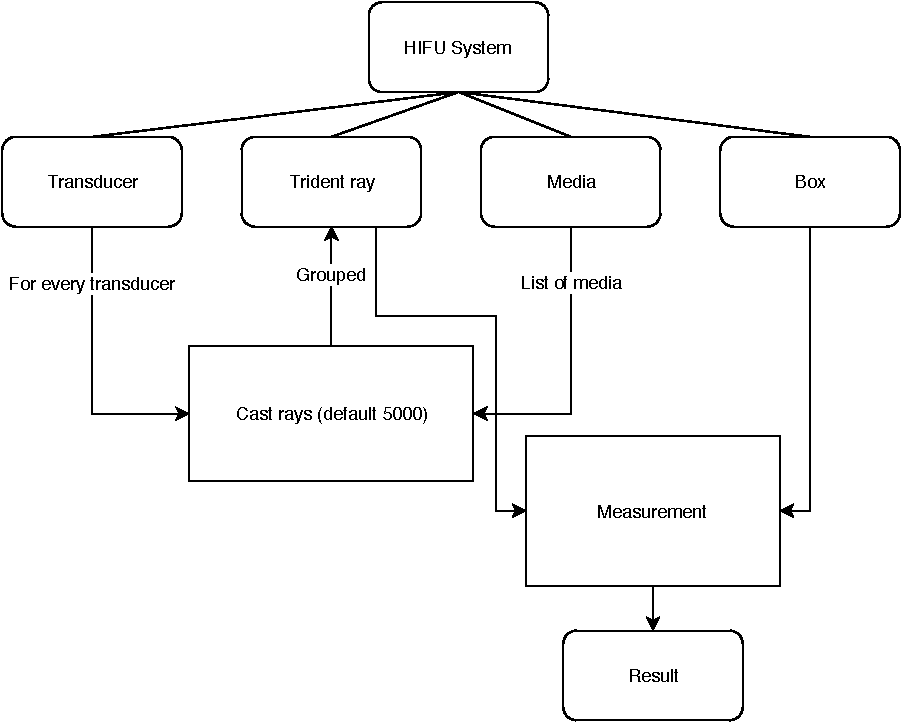
\includegraphics[width=0.6\textwidth]{uml_overview}
    \caption{An overview of all the components in the HIFU system.}
    \label{fig:uml_overview}
\end{figure}

%%%%%%%%%%%%%%%%%%%%
\subsection{Trident}
As mentioned earlier, the ray that carries power is implemented as class \texttt{PowRay} (power ray) and the ray that only helps to determine the divergence is implemented as class \texttt{AuxRay} (auxiliary ray). They both inherit from a general purpose ray class \texttt{Ray}. Class \texttt{Ray} is a subclass of the geometrical ray class \texttt{GeoRay} (Appendix \ref{ap:geometry}), with some properties and methods for acoustics simulation.

A trident ray (class \texttt{Trident}) consists of three rays, one \texttt{PowRay} and two \texttt{AuxRay}s. Every trident have an unique id. Interaction with media doesn't change the id. Member property \code{el\_id} store the id of the transducer where it is casted from. It also have the reference to the media that it reside in. The member property \code{history} records all the media that trident ray has passed through. \code{wavetype} is an int variable that indicates whether the ray is longitudinal or shear wave. A ray can encounter several intersection with media interfaces and produce up to four child rays. Each intersection split the parent rays into reflected rays and transmitted rays, so is the power carried. Once the power of the ray is lower than a predefined threshold \code{powerlimit}, the ray is discarded and the propagation stops.
The trident rays need to be grouped into bundles according to their \code{bundle\_identifier}. \code{bundle\_identifier} is a string that is composed of the id of the transducer the ray originates from, its history and its wavetype. For example, \code{tr\_128\_mh\_0\_1\_1\_1\_LONGIT} can be intepreted as a longitudinal trident casted from transducer element \textit{no.128} propagates from \textit{media 0} into \textit{media 1} then reflects inside  \textit{media 1} twice until its power is lower than \code{powerlimit}.



\begin{lstlisting}[language=Python]
import numpy as np
    
def incmatrix(genl1,genl2):
    m = len(genl1)
    n = len(genl2)
    M = None #to become the incidence matrix
    VT = np.zeros((n*m,1), int)  #dummy variable
    
    #compute the bitwise xor matrix
    M1 = bitxormatrix(genl1)
    M2 = np.triu(bitxormatrix(genl2),1) 
    
    for i in range(m-1):
        for j in range(i+1, m):
            [r,c] = np.where(M2 == M1[i,j])
            for k in range(len(r)):
                VT[(i)*n + r[k]] = 1;
                VT[(i)*n + c[k]] = 1;
                VT[(j)*n + r[k]] = 1;
                VT[(j)*n + c[k]] = 1;
    
                if M is None:
                    M = np.copy(VT)
                else:
                    M = np.concatenate((M, VT), 1)
    
                VT = np.zeros((n*m,1), int)
    
    return M
\end{lstlisting}
    
    
How to init power

how to init phase

how to find next media

how to refract and reflect

how to get intensity, and 3 method to calculate area

how to 
%%%%%%%%%%%%%%%%%%%%%%%
\subsection{Transducer}
A transducer element is a device that can convert other forms of energy into acoustic energy in ultrasound. The transducer in this study consists of 256 transducer elements. In the model, the transducer is implemented as class \texttt{Transducer} and the transducer element is implemented as class \texttt{TElement}.
The mathematical model is written in Python programming language, using scipy suite\cite{scipy}. The visualization of the model is made possible with matplotlib \cite{matplotlib}. The four components mentioned in section \ref{sec:components} will be introduced in detail. A Python class is implemented for each component. This make the program more intuitive and easy to maintain. Other than these four component, the geometry, acoustics are also implemented in object-oriented manner. Class \texttt{HIFU} encapsulates several methods for manipulating the four components above. As is shown in Figure \ref{fig:uml_overview}, \texttt{transducer} casts \texttt{ray} at \texttt{media} and grouped them into bundle according to their properties and history. Then, the grouped rays are sampled on \texttt{box} to get the resulted pressure. The same routine is run for all the transducers. The final result is the summation of the result from all transducer.

\IncMargin{1em}
\begin{algorithm}[H]
    \SetKwData{Left}{left}\SetKwData{This}{this}\SetKwData{Up}{up}
    \SetKwFunction{Union}{Union}\SetKwFunction{FindCompress}{FindCompress}
    \SetKwInOut{Input}{input}\SetKwInOut{Output}{output}
    \Input{parameters, media, box}
    \Output{pressure produced}
    \BlankLine
    \emph{special treatment of the first line}\;
    \For{$i\leftarrow 2$ \KwTo $l$}{
        \emph{special treatment of the first element of line $i$}\;
        \For{$j\leftarrow 2$ \KwTo $w$}{\label{forins}
        \Left$\leftarrow$ \FindCompress{$Im[i,j-1]$}\;
        \Up$\leftarrow$ \FindCompress{$Im[i-1,]$}\;
        \This$\leftarrow$ \FindCompress{$Im[i,j]$}\;
        \If(\tcp*[h]{O(\Left,\This)==1}){\Left compatible with \This}{\label{lt}
            \lIf{\Left $<$ \This}{\Union{\Left,\This}}
            \lElse{\Union{\This,\Left}}
        }
        \If(\tcp*[f]{O(\Up,\This)==1}){\Up compatible with \This}{\label{ut}
            \lIf{\Up $<$ \This}{\Union{\Up,\This}}
            \tcp{\This is put under \Up to keep tree as flat as possible}\label{cmt}
            \lElse{\Union{\This,\Up}}\tcp*[h]{\This linked to \Up}\label{lelse}}
        }
        \lForEach{element $e$ of the line $i$}{\FindCompress{p}}
    }
    \caption{Simulation of one transducer}\label{algo_disjdecomp}
\end{algorithm}
\DecMargin{1em}



config files

ray tracing \cite{wooraytracing}, AABB \cite{smits}

parallelization

line intersection, division handling.

\subsection{Sampling box}
A transducer element is a device that can convert other forms of energy into acoustic energy in ultrasound. The transducer in this study consists of 256 transducer elements. In the model, the transducer is implemented as class \texttt{Transducer} and the transducer element is implemented as class \texttt{TElement}.
The mathematical model is written in Python programming language, using scipy suite\cite{scipy}. The visualization of the model is made possible with matplotlib \cite{matplotlib}. The four components mentioned in section \ref{sec:components} will be introduced in detail. A Python class is implemented for each component. This make the program more intuitive and easy to maintain. Other than these four component, the geometry, acoustics are also implemented in object-oriented manner. Class \texttt{HIFU} encapsulates several methods for manipulating the four components above. As is shown in Figure \ref{fig:uml_overview}, \texttt{transducer} casts \texttt{ray} at \texttt{media} and grouped them into bundle according to their properties and history. Then, the grouped rays are sampled on \texttt{box} to get the resulted pressure. The same routine is run for all the transducers. The final result is the summation of the result from all transducer.

\section{Measurement} \label{sec:measurement}
far field approximation, unit scale \cite{unitscale}

two way to calculate pressure at a box (weighted or unweighted)
